\subsubsection{品質分析・評価技法}

設計品質を分析・評価するための技法には、静的分析、シミュレーション、プロトタイピング、レビュー、要求追跡などがある。

\par\smallskip\noindent\refstepcounter{table}\label{tab:ch03-06}\textbf{表 \thetable: 第03章 ソフトウェア設計 表06}\par\smallskip
\begin{tabularx}{\linewidth}{L{36mm}Y}
\toprule
\textbf{技法} & \textbf{説明} \\
\midrule
設計レビュー・検査 & 設計記述を人が確認し、要求対応、未解決事項、設計上のリスクを見つける。 \\
シナリオに基づく評価 & 利用シナリオ、障害シナリオ、変更シナリオを使って、設計がどう反応するか確認する。 \\
要求追跡 & 要求が設計要素へ対応しているか、設計要素に根拠となる要求があるか確認する。 \\
静的分析 & 実行せずに設計やモデルを分析する。依存関係、循環、整合性、弱点を確認する。 \\
形式的分析 & 数学的モデルを使い、性質を厳密に検査する。安全性やセキュリティが重要な領域で有効である。 \\
シミュレーション & 設計モデルを使い、性能、タイミング、負荷、失敗時の挙動などを試す。 \\
プロトタイピング & 実現可能性、使いやすさ、技術的リスクを確認するために試作品を作る。 \\
\bottomrule
\end{tabularx}

\begin{figure}[htbp]
\centering
\IfFileExists{assets/generated_figures/ch03/fig-ch03-12.png}{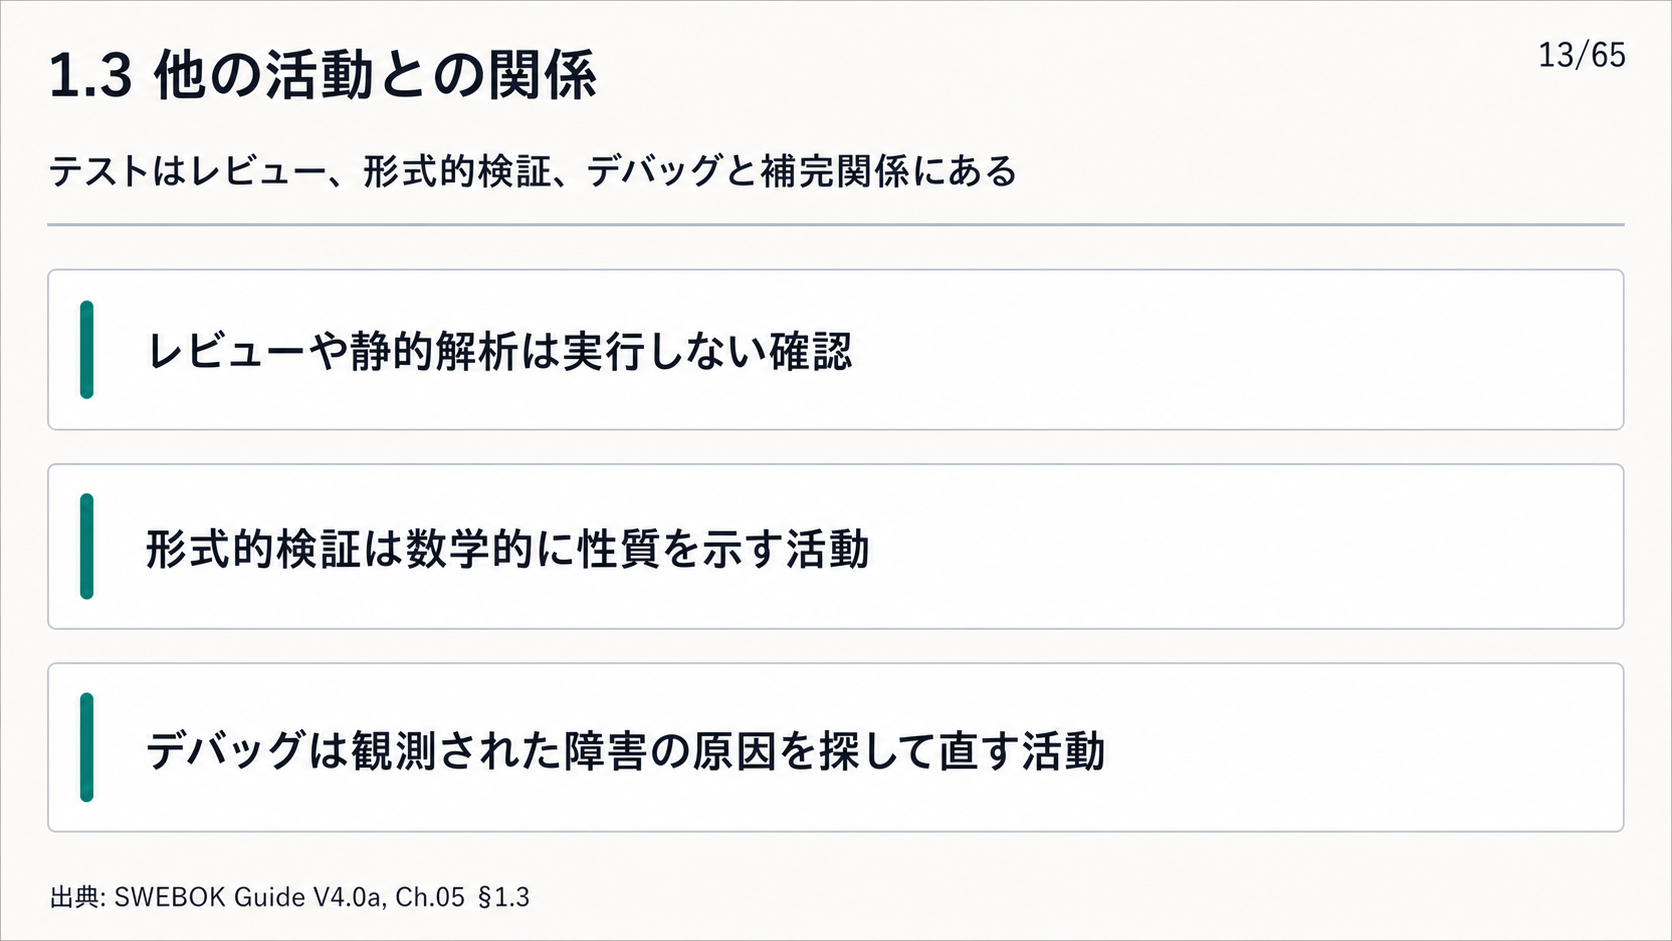
\includegraphics[width=0.96\linewidth]{assets/generated_figures/ch03/fig-ch03-12.png}}{\fbox{\parbox[c][48mm][c]{0.9\linewidth}{\centering 画像生成待ち\\品質分析・評価技法の比較図}}}
\caption{品質分析・評価技法の比較図}
\label{fig:ch03-12}
\end{figure}
